\documentclass[tikz,border=12pt]{standalone}
\usepackage[T1]{fontenc}
\usepackage{mathpazo}
\usepackage{amsmath,amssymb}
\usetikzlibrary{arrows.meta, positioning}

\definecolor{stblue}{HTML}{7B97AD}
\definecolor{rwgold}{HTML}{B8995E}
\definecolor{sage}{HTML}{7A9A7E}
\definecolor{dkbrown}{HTML}{3D3530}
\definecolor{wmgray}{HTML}{7B7067}
\definecolor{cream}{HTML}{F9F6F0}
\definecolor{border}{HTML}{D4C9B8}
\definecolor{rosewood}{HTML}{AD8480}

\begin{document}
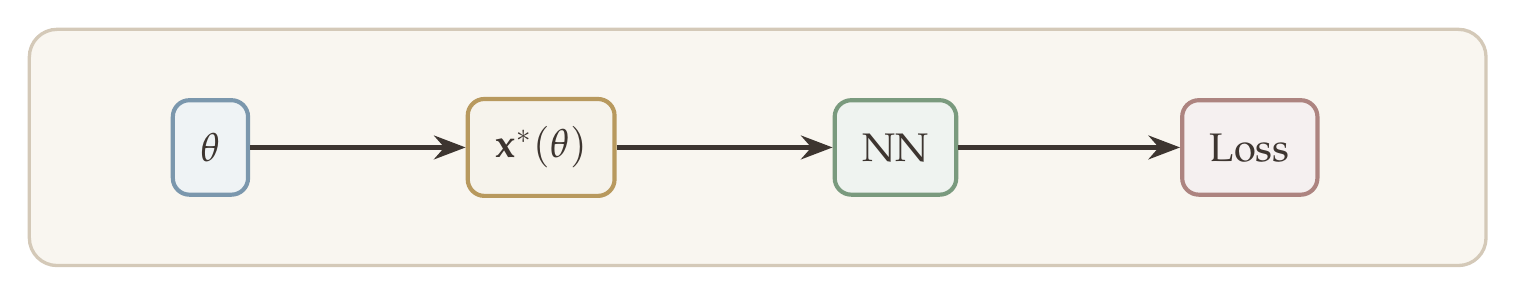
\begin{tikzpicture}[>={Stealth[length=4mm, width=3mm]},
  box/.style={fill=#1!12, draw=#1, line width=1.5pt, rounded corners=6pt,
              minimum height=1.2cm, text=dkbrown, font=\Large,
              align=center, inner sep=10pt}]

% Background
\fill[cream, rounded corners=10pt] (-0.5,-0.5) rectangle (18,2.5);
\draw[border, line width=1.2pt, rounded corners=10pt] (-0.5,-0.5) rectangle (18,2.5);

\node[box=stblue] (theta) at (1.8,1) {$\theta$};
\node[box=rwgold] (xstar) at (6,1) {$\mathbf{x}^*(\theta)$};
\node[box=sage] (nn) at (10.5,1) {NN};
\node[box=rosewood] (loss) at (15,1) {Loss};

\draw[->, dkbrown, line width=2pt] (theta) -- (xstar);
\draw[->, dkbrown, line width=2pt] (xstar) -- (nn);
\draw[->, dkbrown, line width=2pt] (nn) -- (loss);

\end{tikzpicture}
\end{document}
